\documentclass[11pt]{article}
\usepackage{amsmath,amssymb,amsfonts,epsfig,algorithm,algorithmic,url, mathtools, indentfirst, color, soul}

\textheight 8.8truein
\parskip 0.1in
\topmargin -0.5truein
\textwidth 6.5truein
\oddsidemargin -0.05in
\evensidemargin -0.05in
% \renewcommand{\baselinestretch}{1.2}   %line space adjusted here
\setcounter{footnote}{0}
\sloppy

\renewcommand{\theequation}{\thesection.\arabic{equation}}
\newcommand{\newsection}{\setcounter{equation}{0}\section}

% redefining commonly used symbols
\DeclareMathOperator{\trace}{Tr}

\newtheorem{theorem}{Theorem}
\newtheorem{proposition}[theorem]{Proposition}
\newtheorem{lemma}[theorem]{Lemma}
\newtheorem{corollary}[theorem]{Corollary}
\newtheorem{definition}[theorem]{Definition}

\begin{document}
\title{\bf EE394V Power System Operations and Control\\
Learning for DC-OPF: Classifying Active Constraints using Neural Nets 
}
\date{\today}
\author{JeeHyun Park}
%\normalsize{}
\maketitle

%%%%%%%%%%%%%%%%%%%%%%%%%%%%%%%%%%%%%%%%%%%%
% ABSTRACT 
%%%%%%%%%%%%%%%%%%%%%%%%%%%%%%%%%%%%%%%%%%%%
\begin{abstract}
Optimal power flow is used in power system operational planning to estimate the most economical efficiency solution while satisfying demand and safety margins. Due to increasing uncertainty and variability in energy sources and demand, the optimal solution needs to be updated near real-time to respond to observed uncertainty realizations. However, the existing method of solving the optimal problem could not cope with frequent updating due to the high computational complexity. To address this issue, several approaches were introduced to learn the mapping between the uncertainty realization and the optimal solutions. In this paper, we propose the use of neural networks as a classifier learning the mapping between the uncertainty realization and the active constraints set at optimality, which has an extremely low computational complexity. Through experiments, we demonstrate the remarkable performance of this approach and visualize clusters of constraints on systems in the IEEE PES PGLib-OPF benchmark library.
\end{abstract}

%%%%%%%%%%%%%%%%%%%%%%%%%%%%%%%%%%%%%%%%%%%%
% INTRODUCTION
%%%%%%%%%%%%%%%%%%%%%%%%%%%%%%%%%%%%%%%%%%%%
\section{Introduction}\label{sec:intro}
DC optimal power flow (OPF) is one of linear optimization problem to estimate the most economical efficiency solution. Also, the solution satisfies the constraints related to demand and safety. Due to increasing increasing integration of renewable and complexity of demand-side behavior, estimating the solution of DC optimal flow needs to be updated near real-time in response to observed uncertainty realization. 

Traditionally, affine control policy \cite{affine_control1}, \cite{affine_control2}, \cite{affine_control3} was proposed to address frequent updating issue. This method allows re-solving the DC-OPF at a much faster time scale, however it is restrictive and can be sub-optimal in terms of cost and constraints enforcement \cite{affine_control_cons}. Also, the tight latency requirements and large system sizes makes this a computationally challenging task \cite{learning_dc_opf}. 
This motivates the use of machine learning (ML) approaches, called "ensemble policy", to learn the mapping from the uncertainty realization to the optimal solution \cite{statistical_learning}, \cite{learing_constrained_op}. The model of this approach is designed to learn the mapping between uncertainty realization and active constraints. Although direct mapping between uncertainty realization and optimal solution can be used, there is a drawback that the performance of the model depends on the size of the training data set. Assuming the important features, observed in \cite{statistical_learning}, \cite{learing_constrained_op}, that only a few of the constraints are active in the optimal point, adding an estimation of the relevant active constraints as an intermediate stage can guarantee the performance of the model. However, since exhaustive searching is used to estimate relevant active constraints, it has computational a disadvantage that the computational complexity depends on the number of relevant active constraints.

In this paper, we proposed the use of neural network as a classifier to enable extremely low computational complexity compared to the traditional method. In addition, to understand various operational patterns in a given system, we visualized the clustering of constraints that are typically simultaneously active/inactive. 

The rest of the paper is organized as follows. In Section 2, we describe the problem formulation and recap the active-set based approach to learning optimal solutions. In Section 3, we describe the classification method. In Section 4, we describe the design of the experiments and the results. We conclude in Section 5 with directions for future work.

% mapping from uncertainty realization $\omega$ to active constraints set $\mathcal{A^{\star}}$ 

%%%%%%%%%%%%%%%%%%%%%%%%%%%%%%%%%%%%%%%%%%%%
% PROBLEM FORMULATION
%%%%%%%%%%%%%%%%%%%%%%%%%%%%%%%%%%%%%%%%%%%%
\section{Problem Formulation}\label{sec:problem}
\subsection{The case for learning optimal power flow solutions}
We start with DC-OPF under uncertainty conditions as follows.
% power flow problem
\begin{align}\label{eq:opf}
\rho^{\star}\left (  \omega \right )\in \underset{p}{\mathrm{argmin}} \; c^{\top }p \\
\textrm{s.t.} ~ &~ e^{\top }p=e^{\top }\left ( d -\omega  \right ) \\
~&~ p^{min}\leq p\leq p^{max} \\
~&~ f^{min}\leq M\left ( Hp +\omega -d \right )  \leq f^{max}
\end{align}
Here $p$ denotes the vector of dispatchable generator set points, while $c$ is the vector of corresponding linear cost coefficients.  $d$ represents the vector of demands, $\omega$ is the uncertainty realization, and $e$ is the vector of all ones. $H$ is the mapping from generators to their respective buses, and $M$ represents the matrix of power transfer distribution factors (PTDF). The objective (2.1) minimizes generation cost. (2.2) represents the power balance constraint of the system. (2.3) and (2.4) are generator and flow constraints which limits the generation and transmission. Lastly, $\rho$, control policy, is mapping adjusts the generation in response to uncertainty realization. We will set up a control policy model that learns the mapping using given data set and neural networks. The goal of the learning is to estimate $\hat{\rho}$ of the optimal mapping $\rho^{\star}$.

\subsection{Review of the Active-set Approach to Learning Solutions to the DC-OPF}

In the following analysis, we constrict ourselves to the set $\Omega^{R}\coloneqq\left \{ \omega:\mathcal{P}^{\star} \left ( \omega \right )\neq \emptyset \right \}$ of recovery scenarios, i.e., the scenario for which a feasible solution can be found. Since the constraints of DC-OPF are all in linear, the feasible set can be represented by a polytope as in (2.5) and a matrix expression as in (2.6).

% According to \cite{1802.09639}, we could assume the system has $n$ generators, $m$ transmission lines, $v$ buses, and $v$ loads. We set a graph $\mathcal{G}( \mathcal{V}, \mathcal{E})$, where $\mathcal{V}$ denotes the nodes of the graph corresponding to the buses with $\left| \mathcal{V} \right| = v$, and the edges $\mathcal{E}$ denote the transmission lines with $\left| \mathcal{E} \right| = m$.
% A $control \; policy \; \rho : \Omega \rightarrow \mathbb{R}^{n}$ is a mapping that adjusts the generation in response to uncertainty realization $\omega \in \Omega$. 

% polytope
\begin{align}\label{eq:opf_poly}
\mathcal{P}\left ( \omega \right ) =  \{ p\in\mathbb{R}^{n}:
~ &~p^{min}\leq p\leq p^{max}, \nonumber \\
~ &~ f^{min}\leq M\left ( Hp +\omega -d \right )  \leq f^{max}, \nonumber \\
~ &~ e^{\top }p=e^{\top }\left ( d -\omega  \right )  \}
\end{align}

% opf in compact matrix
\begin{align}\label{eq:opf_poly_compact}
\mathcal{P}\left ( \omega \right ) =  \{ p:
~ &~ Ap\leq b+C\omega, \; e^{\top }p=e^{\top }\left ( d -\omega  \right )  \}, \\
\text{where}
~ &~ A=\begin{bmatrix}I\\ -I\\ MH\\ -MH\end{bmatrix} \in \mathbb{R}^{2\left(n+m\right)\times n},
~ &~ C=\begin{bmatrix}0\\ -0\\ M\\ -M\end{bmatrix} \in \mathbb{R}^{2\left(n+m\right)\times v}, \nonumber \\
~ &~ b=\begin{bmatrix}p^{max}\\ -p^{min}\\ f^{max}+Md\\ -f^{min}+Md\end{bmatrix} \in \mathbb{R}^{2\left(n+m\right)}. \nonumber
\end{align}

In \cite{statistical_learning} and \cite{learing_constrained_op}, we obtained following two key observations; (i) For typical uncertainty distributions of the random vector ω, only a few of the active sets are realized, and (ii) The optimal solutions to linear programs lie at extreme points of the feasible polytope. If these two key points are always assumed to be true, we can get the optimal solution as shown in (2.7).

% optimal solution
\begin{align}\label{eq:opf_affine}
p^{\star}=B^{-1}\begin{bmatrix}
b_{\mathcal{A}}+C_{\mathcal{A}}\omega\\ 
e^{\top}\left(d-\omega\right)
\end{bmatrix} \coloneqq\rho^{\mathcal{A}}\left(\omega\right) \\
\text{where}
~ &~ B=\begin{bmatrix} A_{\mathcal{A}}\\ e^{\top} \end{bmatrix} \nonumber \\
~ &~ \mathcal{A} = \left \{ i_{1}, i_{1}, ..., i_{n-1} \right \}, \nonumber \\
~ &~ A_{\mathcal{A}} \coloneqq \text{the sub-matrix of } A \text{ formed by row in } \mathcal{A}, \nonumber \\
~ &~ b_{\mathcal{A}} \coloneqq \text{the sub-vector of } b \text{ formed by row in } \mathcal{A}, \nonumber \\
~ &~ C_{\mathcal{A}} \coloneqq \text{the sub-matrix of } C \text{ formed by row in } \mathcal{A}. \nonumber
\end{align}

By drawing sufficiently many samples of $\omega$ from the uncertainty distribution $\mathbb{P}_{\omega}$ and solving the optimal problem with (2.7), we could obtain important active constraints of the given system. In \cite{learing_constrained_op}, a stopping criterion is described to ensure that the number of $\omega$ samples is sufficiently large to discover most of the important active constraints set denoted by $I$.  Once the important active sets $I$ is obtained, for a new uncertainty realization $\omega$, the optimal solution can be estimated by (2.8), called ensemble policy using exhaustive search. 

% ensemble policy
\begin{align}\label{eq:ensemble_policy}
\hat{\rho}\left(\omega\right) & \coloneqq \underset{\rho^{\mathcal{A}}\left(\omega\right):\mathcal{A}\in I}{\mathrm{argmin}} \; c^{\top}\rho^{\mathcal{A}}\left(\omega\right) \\
\textrm{s.t.} 
~ &~ \rho^{\mathcal{A}}\left(\omega\right) \in \mathcal{P}\left(\omega\right) \nonumber
\end{align}


\subsection{Learning Optimal Solution by Classification of Active Constraints}
The computational complexity of the ensemble policy (2.8) is determined by the number of important active sets $\left| I \right|$. Ensemble policy is an attractive choice if $\left| I \right|$ is small. However, when $\left| I \right|$ is become large, the computational burden can be large making real-time solution updating impossible. 

In \cite{learning_dc_opf}, a neural networks (NNs) classifier was employed instead of exhaustive search, which solved the issue of computaional complexity. This classifier focuses only on important constraint sets. It takes $\omega$ as an input argument and returns a probability vector as output, and we could obtain an optimal solution using the active set having highest probability. In a nutshell, this classifier is used to select which of the important constraints to be active.

In this paper, We also use the NNs classifier. However, the classifier focuses on all the constraints. It takes $\omega$ as an input argument and returns a vector with dimensions equal to the number of the constraints. This vector consists only of 0s and 1s, which represent inactive (0) and active (1). 
The advantage of this modified classifier is that, like the classifier used in 1, active constraints for estimating optimal solution can be obtained, and information about inactive constraints can also be directly obtained. Through this, we can improve our understanding of various operational patterns in a given system. However, since this classifier has a relatively high dimension of output, prediction performance may be deteriorated.
In Section 4, We verified operational patterns through experiments and checked if performance degradation occurs.

% We employ the classification algorithm to learn the mapping from uncertainty realization $\omega$ to the corresponding active constraint set $\mathcal{A}^{\star}\left( \omega \right)$. We use neural network to build a classifier $\hat{\rho}$, the details are described in 2.2. The followings are metrics of the performance of the classifier.


%%%%%%%%%%%%%%%%%%%%%%%%%%%%%%%%%%%%%%%%%%%%
% CLASSIFICATION
%%%%%%%%%%%%%%%%%%%%%%%%%%%%%%%%%%%%%%%%%%%%
\section{Classification}\label{sec:classication}

\begin{figure}[h]\label{fig:nns_arch}
\centering
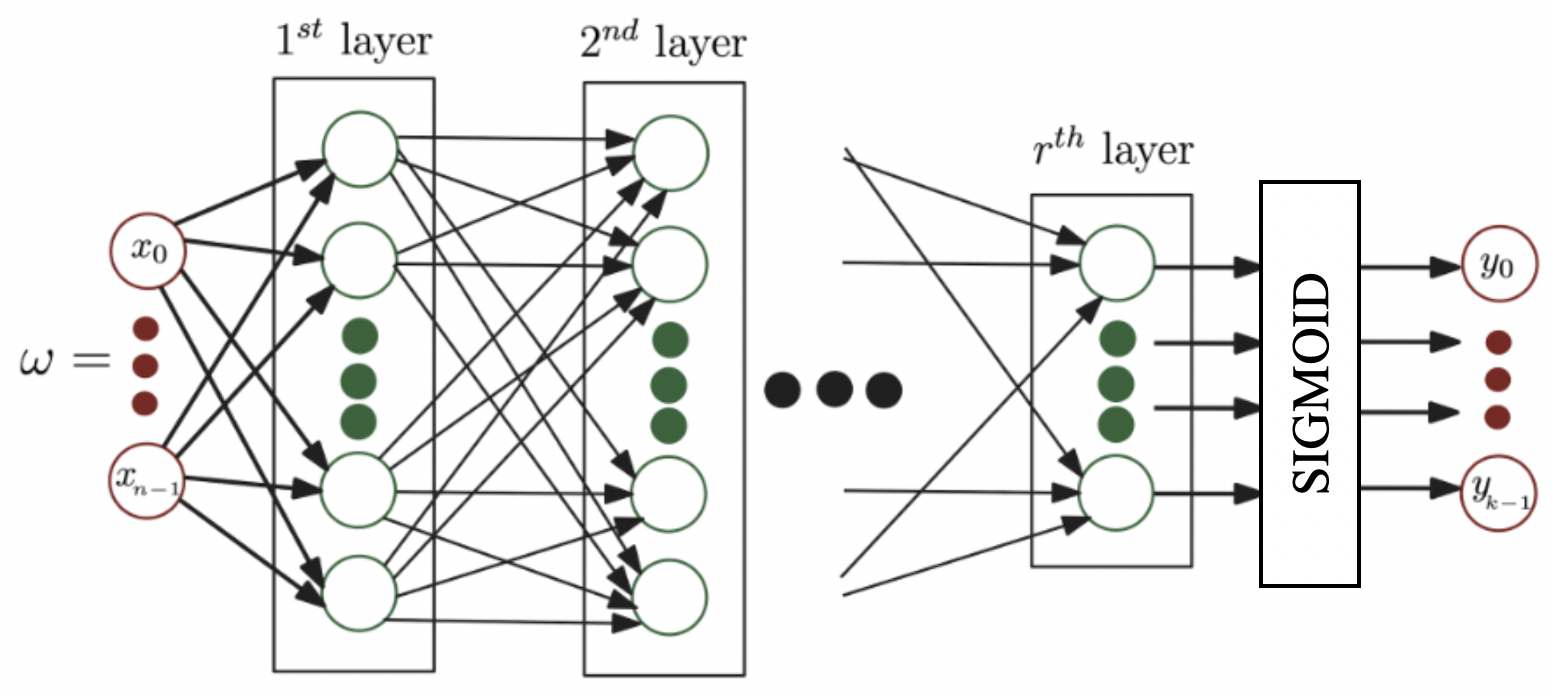
\includegraphics[scale=0.5]{report/figure/NNs_arch.png}
\caption{Architecture of the Neural Network Classifier.}
\end{figure}

We use a simple multi-Dense layer neural networks for our classification task. The generic structure of the classifier is shown in Figure 1. This classifier receives $\omega$ as an input argument $x$, and $y$ returned as output is a binary vector representing active/inactive of each constraints. It should be noted that the activation function of each layer is ReLUs (Rectified Linear Units), but the sigmoid function must be the activation function in the last layer to receive binary output. In addition, to eliminate the issue of covariance shift and regularizing issue, we use batch normalization\cite{batch_norm} and dropout\cite{dropout} for each Dense layer. We use binary cross entropy\cite{bin_cross_entropy} as a loss function and Adam\cite{adam} as an optimizer.


%%%%%%%%%%%%%%%%%%%%%%%%%%%%%%%%%%%%%%%%%%%%
% EXPERIMENTS AND RESULTS
%%%%%%%%%%%%%%%%%%%%%%%%%%%%%%%%%%%%%%%%%%%%
\section{Experiments and Results}\label{sec:experiment_result}
\subsection{Experiments}
In this paper, the data sets of the IEEE PES PGLib-OPF benchmark library \cite{pglib-opf} were used for the experiment. Test case are listed in Table 1. As in \cite{learning_dc_opf}, we assume that the loads are uncertain, and that $\omega$ follow a multivariate normal distribution with mean zero and standard deviation $\sigma$ proportional to the loads, i.e., $\sigma_{i} = 0.03*d_{i}$. We draw 50,000 independent samples and split into three sets, train, validate, and test set.  

\subsection{Results}
Table 1 shows the binary accuracy and binary cross entropy results for each test case. It was expected that the performance of the classification model would decrease as the output dimension increased, but this did not occur. This is expected because the mapping that needs to be learned is relatively simple. It is expected that the decrease in performance can be observed when the system complexity increases due to the increase in the size of the given system and the number of transmission lines. 

Figure 2 is heat-maps visualizing the distribution of active constraints for each test case. In this heat map, 1 appearing in white stands for the constraint is active, and 0 appearing in red means inactive. The values corresponding to -1 appearing in black are meaningless data added to construct a heat map. 
First of all, it was confirmed that the predict result of the classification model matches the actual value. Also, operational patterns in a given system, such as clustering of constraints was checked. However, we could only check the cluster of constraints by this results, and it is unknown whether there is a correlation between uncertainty realization and constraints. If mapping between uncertainty realization and constraints can be traced, it can be used for locational marginal price (LMP) prediction.



\begin{table}[h]
\centering
\begin{tabular}{|r|r|r|}
\hline
        & BinaryAccuracy & BinaryCrossEntropy \\ \hline
24 bus  & 0.99           & 0.00116            \\ \hline
57 bus  & 0.99           & 0.00056            \\ \hline
162 bus & 0.99           & 0.00039            \\ \hline
300 bus & 1.00           & 0.00026            \\ \hline
\end{tabular}
\caption{Accuracy and Loss Results of each Experiments}
\end{table}


\begin{figure}[h!]\label{fig:visualization_results}
\centering
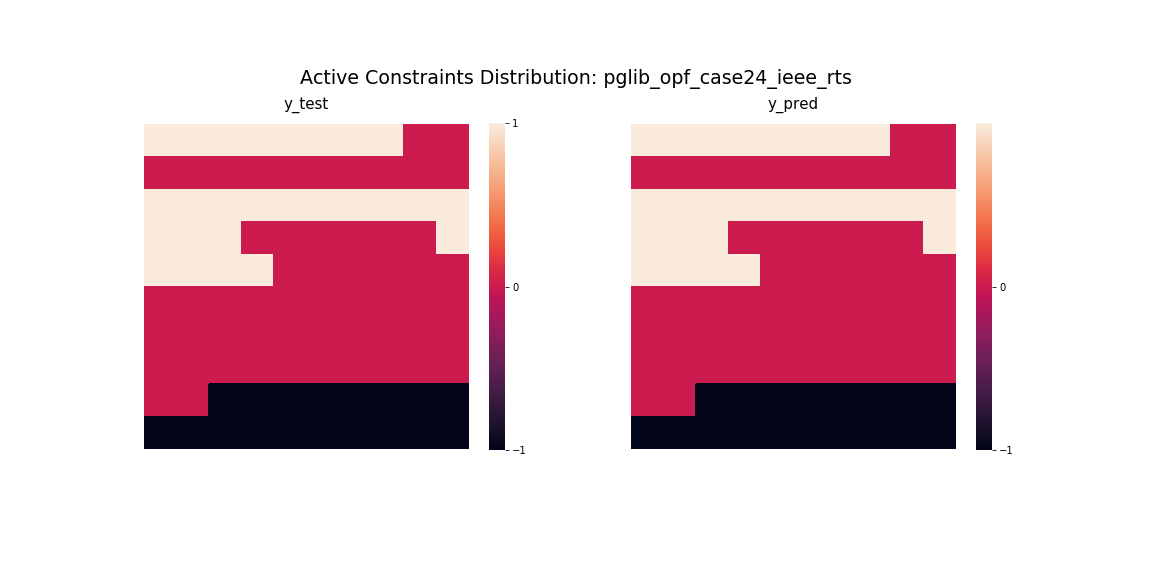
\includegraphics[scale=0.253]{codes/experiments/figures/pglib_opf_case24_ieee_rts.png}
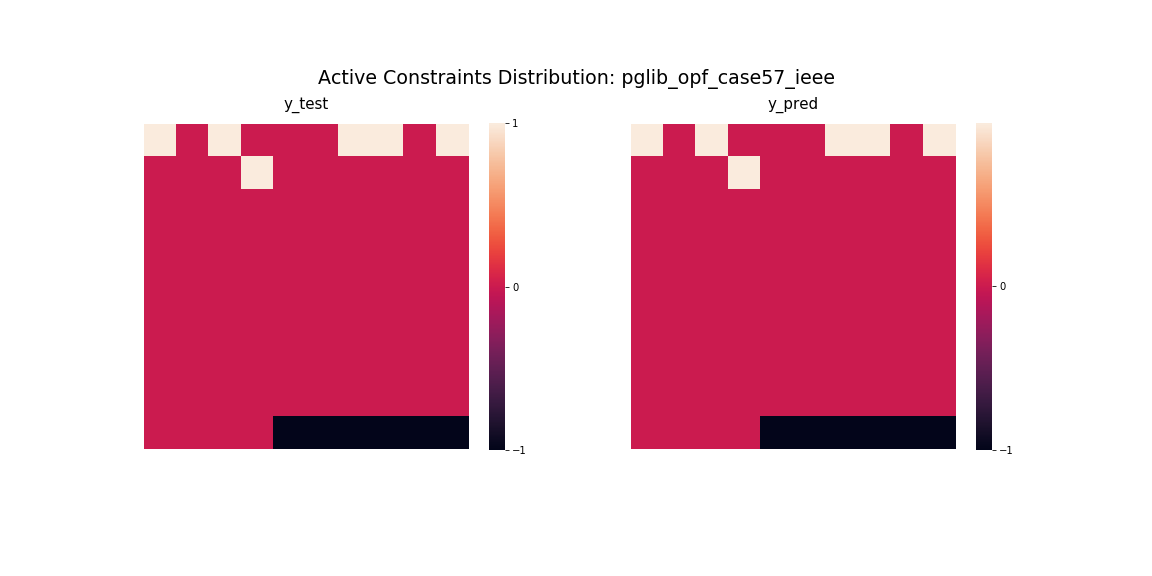
\includegraphics[scale=0.253]{codes/experiments/figures/pglib_opf_case57_ieee.png}
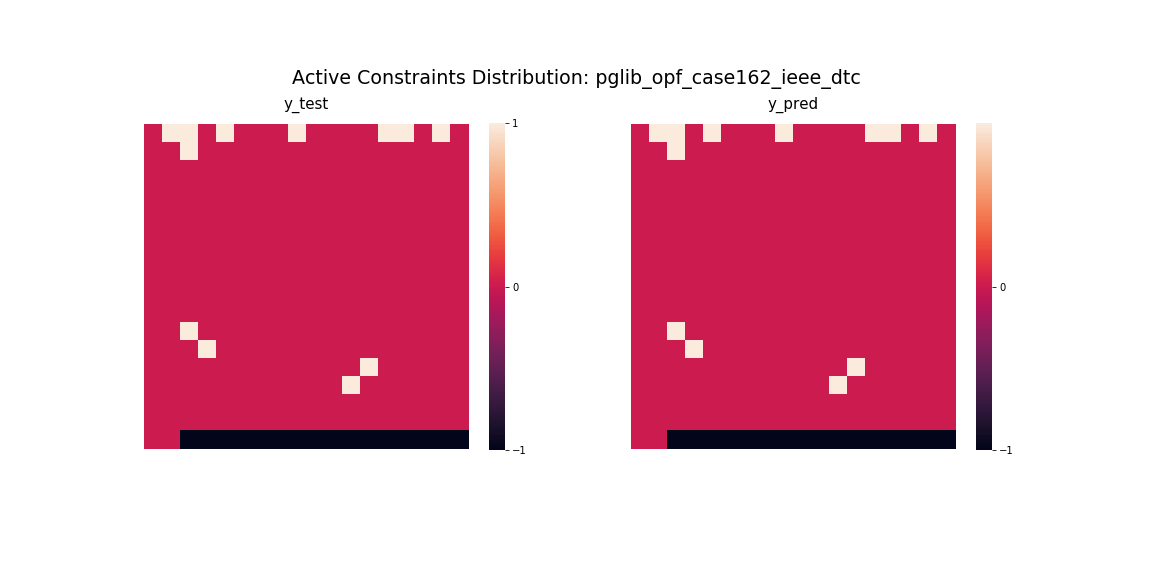
\includegraphics[scale=0.253]{codes/experiments/figures/pglib_opf_case162_ieee_dtc.png}
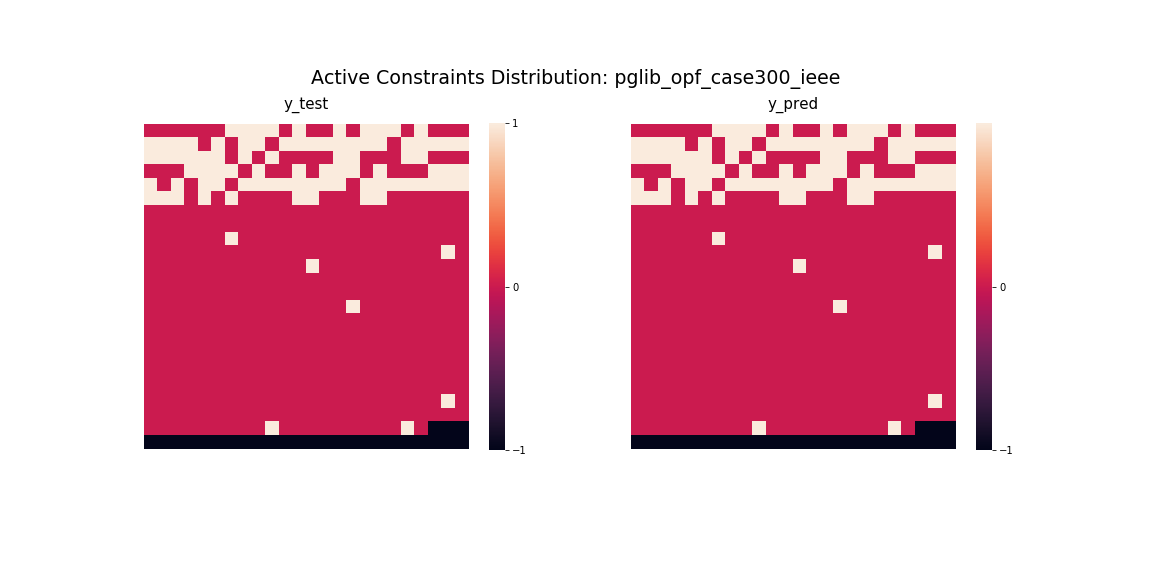
\includegraphics[scale=0.253]{codes/experiments/figures/pglib_opf_case300_ieee.png}
\caption{Visualization of active & inactive constraints distribution.}
\end{figure}

%%%%%%%%%%%%%%%%%%%%%%%%%%%%%%%%%%%%%%%%%%%%
% CONCLUSIONS AND FUTURE WORK
%%%%%%%%%%%%%%%%%%%%%%%%%%%%%%%%%%%%%%%%%%%%
\section{Conclusions and Future Work }\label{sec:conclusions}
The NNs classifier for selecting active constraints proposed in this paper showed very high computational efficiency and satisfactory prediction accuracy. Compared to the method proposed in \cite{learning_dc_opf}, there was concern about the performance degradation of the classifier, but as a result of the experiment, the performance did not decrease.
Through this approach, the optimal solution can be updated near real-time. Also, it was possible to confirm operational patterns, such as clustering of constraints, in a given system through the results of the classifier. This is expected to help in developing tools for operational planning and real-time control. Furthermore, it would be more useful if weight mapping between uncertainty realization and constraints could be obtained. To specific, this mapping can be used in LMP prediction. It is expected to be obtained through Transformer\cite{transformer}, one of the attention algorithms in natural language process.

% In this section, we will discuss whether the performance of classification is satisfactory and whether online updating is possible due to the reduced computational complexity. As further studies, we will discuss \hl{how to extend the proposed method to AC OPF with non-linear variations}. Also, we will discuss about \hl{setting a set of parallel binary classifiers to predict the status of individual constraints separately, which will be an approach to develop a deeper understanding of various operational patterns, such as clustering of constraints.} 

%%%%%%%%%%%%%%%%%%%%%%%%%%%%%%%%%%%%%%%%%%%%
% REFERENCE
%%%%%%%%%%%%%%%%%%%%%%%%%%%%%%%%%%%%%%%%%%%%
\begin{thebibliography} {TL99}

\bibitem{affine_control1} 
{\sc B. Borkowska,} 
"Probabilistic Load Flow," in IEEE Transactions on Power Apparatus and Systems, vol. PAS-93, no. 3, pp. 752-759, May 1974, doi: 10.1109/TPAS.1974.293973.

\bibitem{affine_control2} 
{\sc Maria, Margellos, Kostas, Lygeros, John, Andersson, and Göran,} 
“Probabilistic guarantees for the N-1 security of systems with wind power generation,” Reliability and risk evaluation of wind integrated power systems, 01-Jan-1970. [Online]. Available: https://www.research-collection.ethz.ch/handle/20.500.11850/78417. [Accessed: 10-May-2020].

\bibitem{affine_control3} 
{\sc L. Roald, S. Misra, T. Krause and G. Andersson,} 
"Corrective Control to Handle Forecast Uncertainty: A Chance Constrained Optimal Power Flow," in IEEE Transactions on Power Systems, vol. 32, no. 2, pp. 1626-1637, March 2017, doi: 10.1109/TPWRS.2016.2602805.

\bibitem{affine_control_cons}
{\sc L. Roald, S. Misra, M. Chertkov and G. Andersson,} 
"Optimal Power Flow with Weighted chance constraints and general policies for generation control," 2015 54th IEEE Conference on Decision and Control (CDC), Osaka, 2015, pp. 6927-6933, doi: 10.1109/CDC.2015.7403311.

\bibitem{learning_dc_opf} 
{\sc D. Deka and S. Misra,} 
"Learning for DC-OPF: Classifying active sets using neural nets," 2019 IEEE Milan PowerTech, Milan, Italy, 2019, pp. 1-6, doi: 10.1109/PTC.2019.8810819.

\bibitem{}
{\sc R. D. Christie, B. F. Wollenberg and I. Wangensteen,} 
"Transmission management in the deregulated environment," in Proceedings of the IEEE, vol. 88, no. 2, pp. 170-195, Feb. 2000, doi: 10.1109/5.823997.

\bibitem{statistical_learning}
{\sc Y. Ng, S. Misra, L. A. Roald and S. Backhaus,} 
"Statistical Learning for DC Optimal Power Flow," 2018 Power Systems Computation Conference (PSCC), Dublin, 2018, pp. 1-7, doi: 10.23919/PSCC.2018.8442859.

\bibitem{learing_constrained_op}
{\sc Misra, Roald, and Yeesian,} 
“Learning for Constrained Optimization: Identifying Optimal Active Constraint Sets,” arXiv.org, 16-Jan-2019. [Online]. Available: https://arxiv.org/abs/1802.09639. [Accessed: 10-May-2020].

\bibitem{batch_norm}
{\sc Sergey, }
“Batch Normalization: Accelerating Deep Network Training by Reducing Internal Covariate Shift,” arXiv.org, 02-Mar-2015. [Online]. Available: https://arxiv.org/abs/1502.03167. [Accessed: 10-May-2020].

\bibitem{dropout}
{\sc N. Srivastava, G. Hinton, A. Krizhevsky, I. Sutskever, and R. Salakhutdinov,} 
“Dropout: A Simple Way to Prevent Neural Networks from Overfitting,” Journal of Machine Learning Research, 01-Jan-1970. [Online]. Available: http://jmlr.org/papers/v15/srivastava14a.html. [Accessed: 10-May-2020].

\bibitem{bin_cross_entropy}
{\sc }
“Binary crossentropy loss function: Peltarion Platform,” Peltarion.com. [Online]. Available: https://peltarion.com/knowledge-center/documentation/modeling-view/build-an-ai-model/loss-functions/binary-crossentropy. [Accessed: 05-May-2020]

\bibitem{adam}
{\sc Kingma, D. P., Jimmy, and Ba,} 
“Adam: A Method for Stochastic Optimization,” arXiv.org, 30-Jan-2017. [Online]. Available: https://arxiv.org/abs/1412.6980. [Accessed: 10-May-2020].

\bibitem{pglib-opf}
Power-Grid-Lib, “power-grid-lib/pglib-opf,” GitHub, 03-Sep-2019. [Online]. Available: https://github.com/power-grid-lib/pglib-opf. [Accessed: 10-May-2020].

\bibitem{transformer}
{\sc Vaswani, Ashish, Shazeer, Noam, Parmar, Niki, Jakob, Jones, Gomez, A. N., Kaiser, Lukasz, Polosukhin, and Illia,}  
“Attention Is All You Need,” arXiv.org, 06-Dec-2017. [Online]. Available: https://arxiv.org/abs/1706.03762. [Accessed: 10-May-2020].

% \bibitem{}
% {\sc }




\end{thebibliography}

\end{document}
